\section{Results}
Particularly Suicide watch community consists of over 78k subscribers and reader, however is supported by mere 12 Moderators according to the latest count. The moderators are mainly present to prevent any kind of abuse, trolling or non-clinical or non-productive advices. These moderators do not have any form of formal training. However through several accounts they have confessed to learn through interactions and mentorship from more senior moderators on the site\footnote{\url{https://bbc.in/24rJYQH}} All the moderators have been in that role for at least 3 years and the oldest goes as far as December 2008. 

Our study is based on all conversations on SuicideWatch.
We represent these conversations through networked abstractions as described in \ref{Sec:Abstractions}.

Through our analysis we find several discriminatory factors among Suicide watch conversations and generic front page conversation. We show that some of these factors are predictive of suicide watch conversations to a very high degree. We also show that certain properties of these conversations can be backed by sociological theories of real life support conversations. 

\subsection{Peculiarity of threads of Support}
We begin by characterizing the two networked abstractions, namely Reply Graphs and Interaction graphs as described in Section \ref{Sec:Abstractions}. 
We do so by first comparing these two abstractions with a baseline control conversation threads using certain macroscopic network properties. 
We first compare the number of unique users per thread. The two communities exhibit considerable difference. SW Sub-Reddit has a median of 5 users per thread and a mean of 6.7 users and BL threads have a median of 25 users and mean of 50 unique users. So this off the bat indicates that Suicide watch conversations are more intimate and involve less participants. Authors tend to participate on a similar level, with a median participation per author of Suicide Watch to be 5 and for baseline conversations to be 3.

\subsubsection{How urgent are user responses?}
Understanding the inter message times can act as a good proxy for the urgency in a conversation. To understand how Suicide watch subreddit users responds to a $OP$ compared to other sub-reddit threads on the frontpage, we calculate differences between the posting times between consecutive messages in a reply graph. Figure \ref{fig:urgency} shows comparison using CDFs of inter-message response times for SW and FP threads. It can be seen that SW $OP$ are responded with the highest urgency amongst the 4, especially compared to either the $OP$ or any other users or sub-reddits. 

\begin{figure}[!ht]
	\centering
	% \hspace*{-5mm}
	\subfloat[]{
		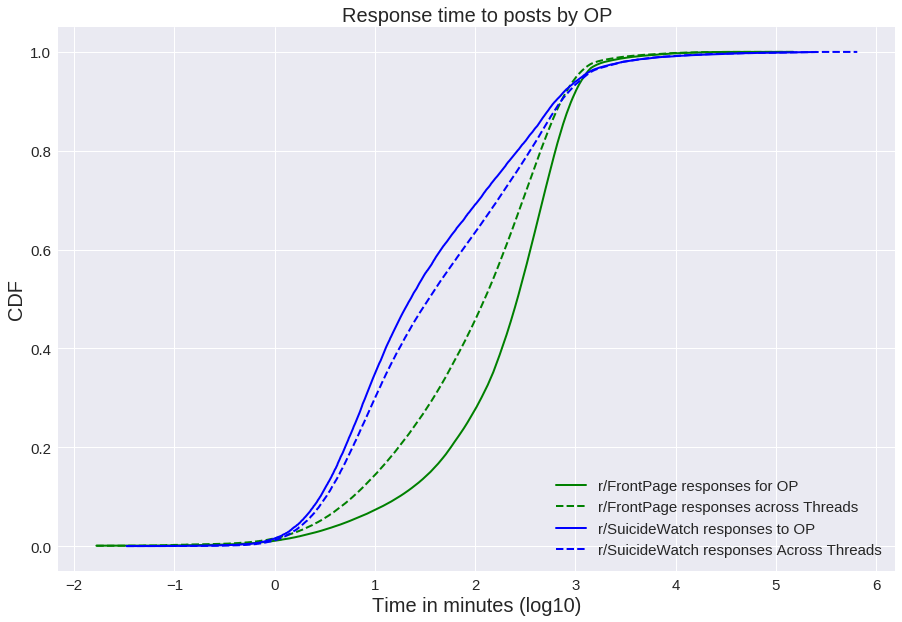
\includegraphics[width=0.4\textwidth ]{Figures/respTimeDist.png}
		\label{fig:urgency}
	}
	\subfloat[]{
		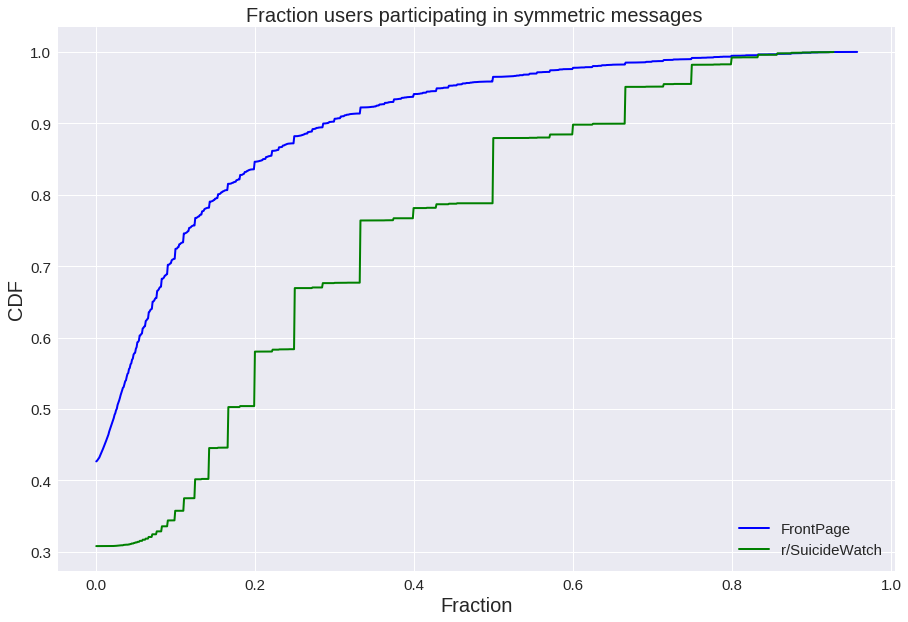
\includegraphics[width=0.4\linewidth ]{Figures/SymUsers.png}
		\label{fig:sym}
	}
    
    \subfloat[]{
		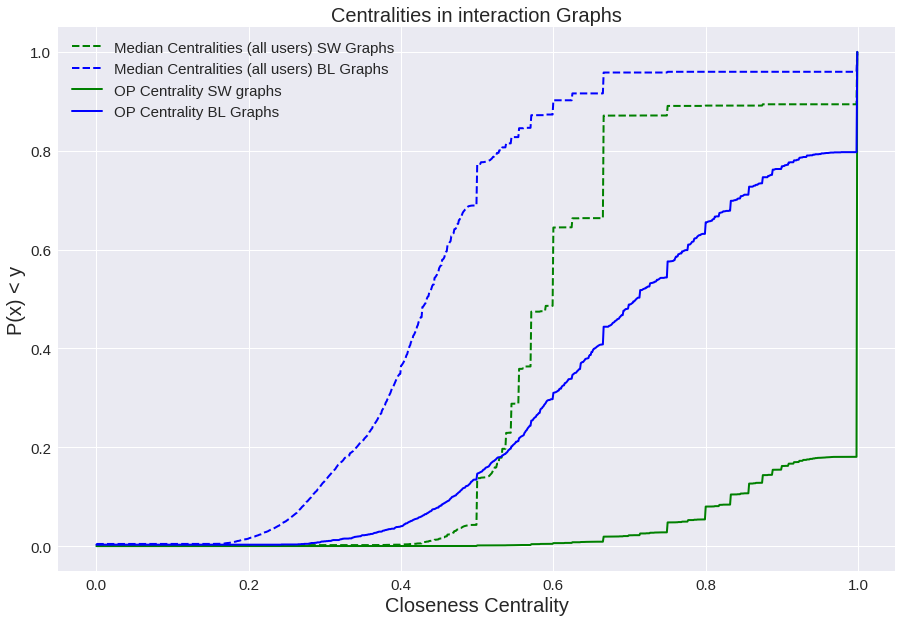
\includegraphics[width=0.4\linewidth ]{Figures/AllCentralities.png}
		\label{fig:centrality}
	}
    \subfloat[]{
		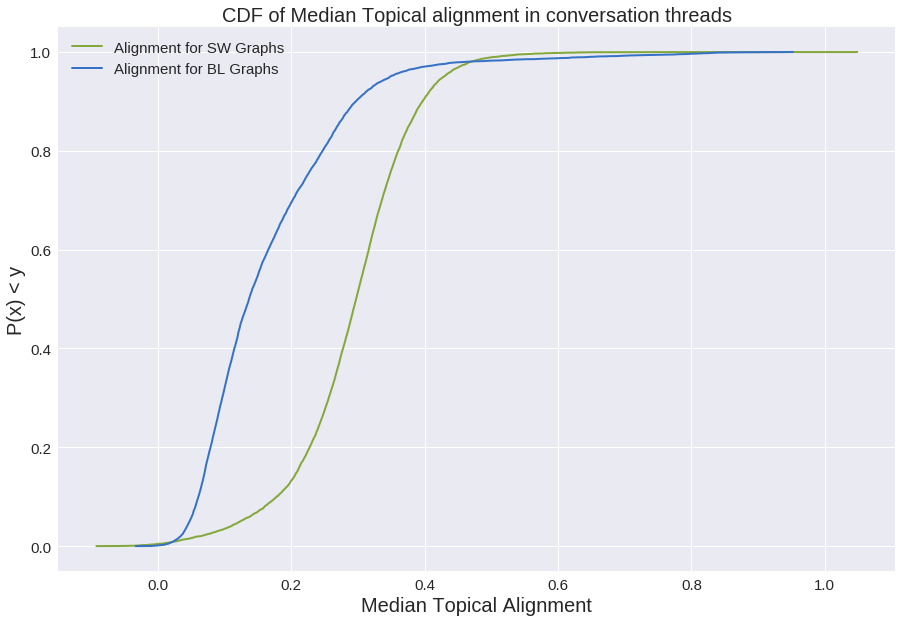
\includegraphics[width=0.4\linewidth ]{Figures/medianTA.png}
		\label{fig:topical}
	}
    
    \subfloat[]{
		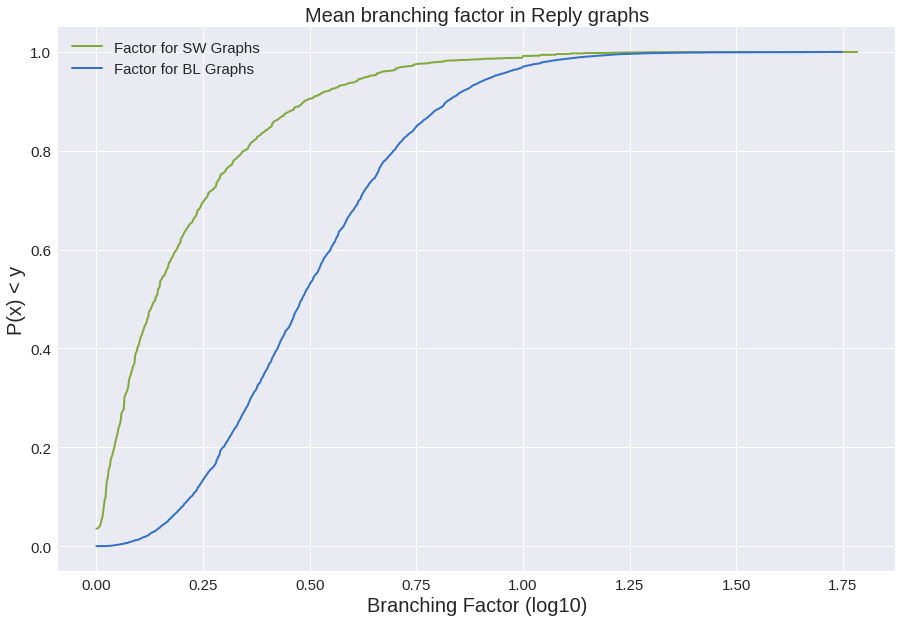
\includegraphics[width=0.4\linewidth ]{Figures/meanBranchingFactor.png}
		\label{fig:branching}
	}
    \subfloat[]{
		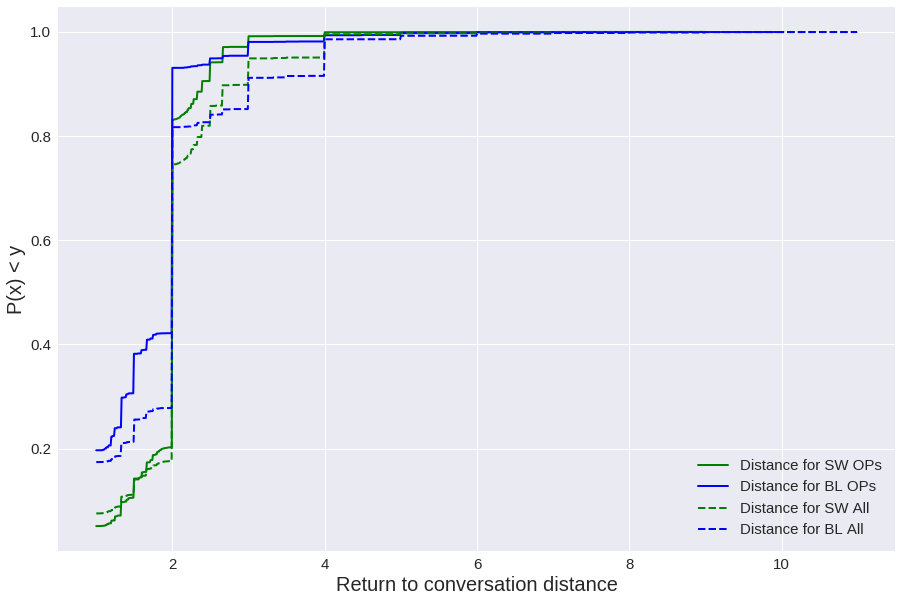
\includegraphics[width=0.4\linewidth ]{Figures/returnDistance.png}
		\label{fig:returndist}
	}
    
    
\caption{Panel shows CDFs of different network metrics. Fig.\ref{fig:urgency} shows the response time distributions, Fig.\ref{fig:sym} shows symmetrically engaged users, Fig.\ref{fig:topical} shows topical similarities across posts and \ref{fig:branching} shows the branching factors of reply graphs. }
\end{figure}

\subsubsection{How symmetric are the interactions?}
Despite signs of urgency and engagement, we ask the question: what percentage of conversations happening on these subreddits are symmetric in nature ? 
For this The median value for $U_{sym}$ for SW is 20\% where as for AS is 0\%. This shows that SW subreddit engages is a lot more symmetric conversation that the baseline threads.
If we define a set of users who engage in symmetric activity with the $OP$ , it would be worth while to investigate how much of the total message activity on the thread is carried out by these set of symmetric users . To calculate this we find the fraction of messages on each thread written as part of this symmetric conversation. Figure \ref{fig:sym} shows the trend. It can be see that SW threads contain a higher prevalence of symmetric message exchanges compared to the baseline Frontpage threads. This shows a higher engagement from the $OP$s side when participating in a supportive conversations

\subsubsection{How central are the users?}
To understand how embedded is the $OP$ in a conversation thread, we compare the betweenness centralities of $OPs$ in the $SW$ dataset with the baseline $FP$ dataset. 
Betweenness centrality is a good proxy of understanding how closely linked is a node with the rest of the network. When we calculate this metric for the user graphs we see that Suicide watch $OP$s tend to have highest centralities compared to generic $FP$ threads moth in terms of $OP$ centrality as well as median centrality across all the users. The high centrality of $OP$s in $SW$ conversations implies a high level of embedded-ness as well as a $OP$ centric approach by other participants in the conversation. The Figure \ref{fig:centrality} shows the Empirical CDFs of centralities. 

\subsubsection{How semantically aligned are the responses?}
We measure semantic alignment based on word embeddings of the source post and the reply post, at every edge of the reply graph. The detailed method of extracting semantic alignment along a post and its response is described in Section \ref{Sec:Semantic}. Extracting such similarity metrics, we compare the trend in response text being in semantic alignment with the parent text in the reply graphs. 


\subsubsection{How branched do conversations become?}
Branching in a conversation thread could be either a sign of digression or a sign interestingness resulting in more people joining in. To measure this phenomena, use the reply graphs, which resemble a n-ary directed acyclic graph, to evaluate the branching factor. 

\subsubsection{How often do users come back to respond ? }



\subsection{Patterns in local interactions}
To answer this question, we use a method more commonly known as network motif analysis to understand triads, or groups of three nodes, and the patterns of edges that exist between them. 

\begin{figure}[!ht]
	\centering
	% \hspace*{-5mm}
% 	\subfloat[]{
% 		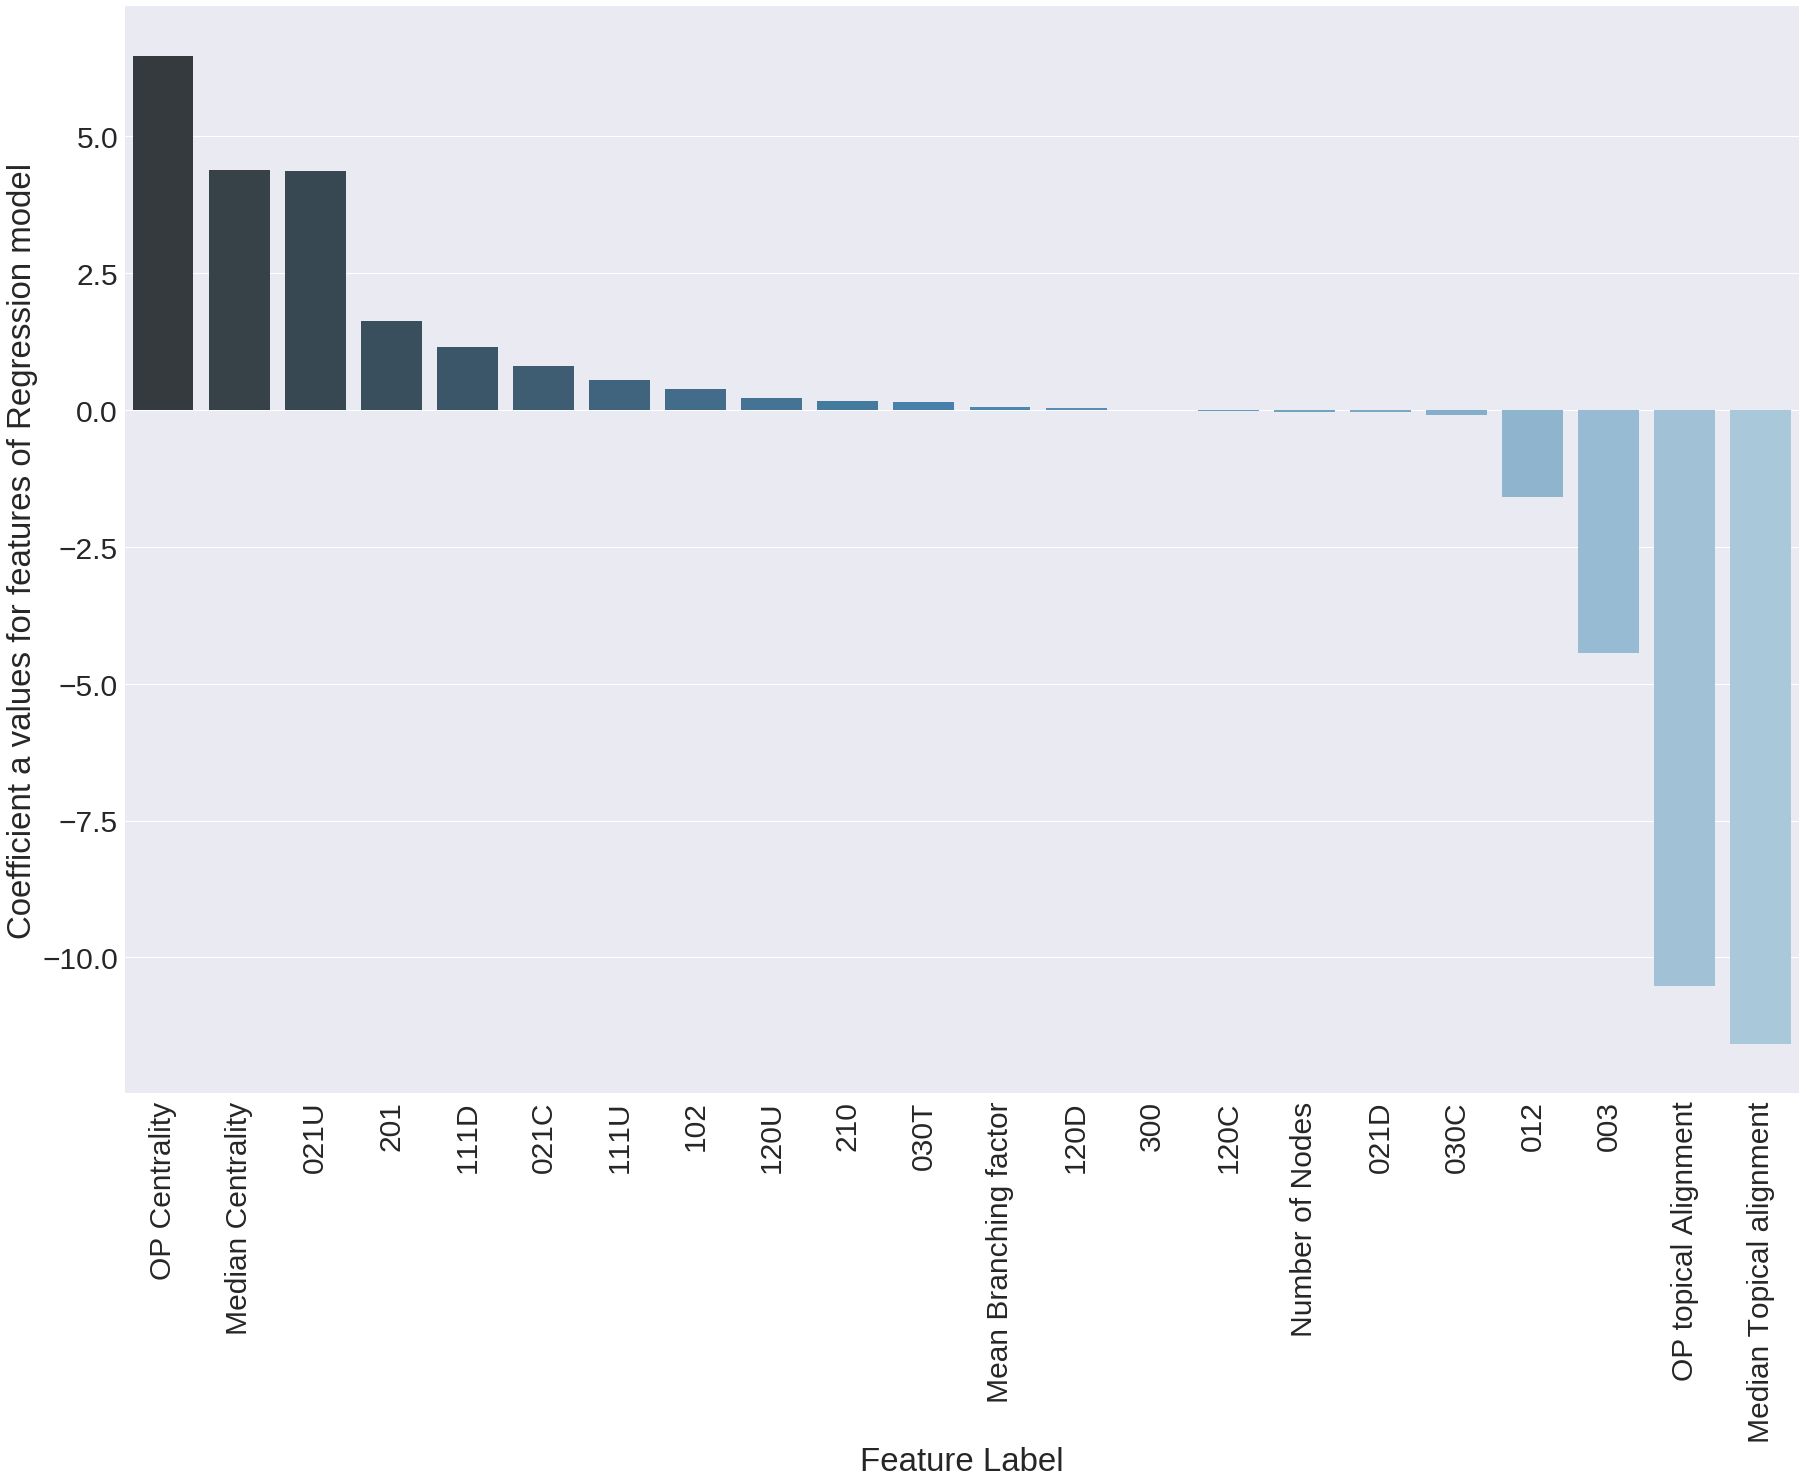
\includegraphics[width=0.5\textwidth, height = 6cm ]{Figures/RevisedFeatureRegression.png}
% 		\label{fig:feats}
% 	}
% 	\subfloat[]{
% 		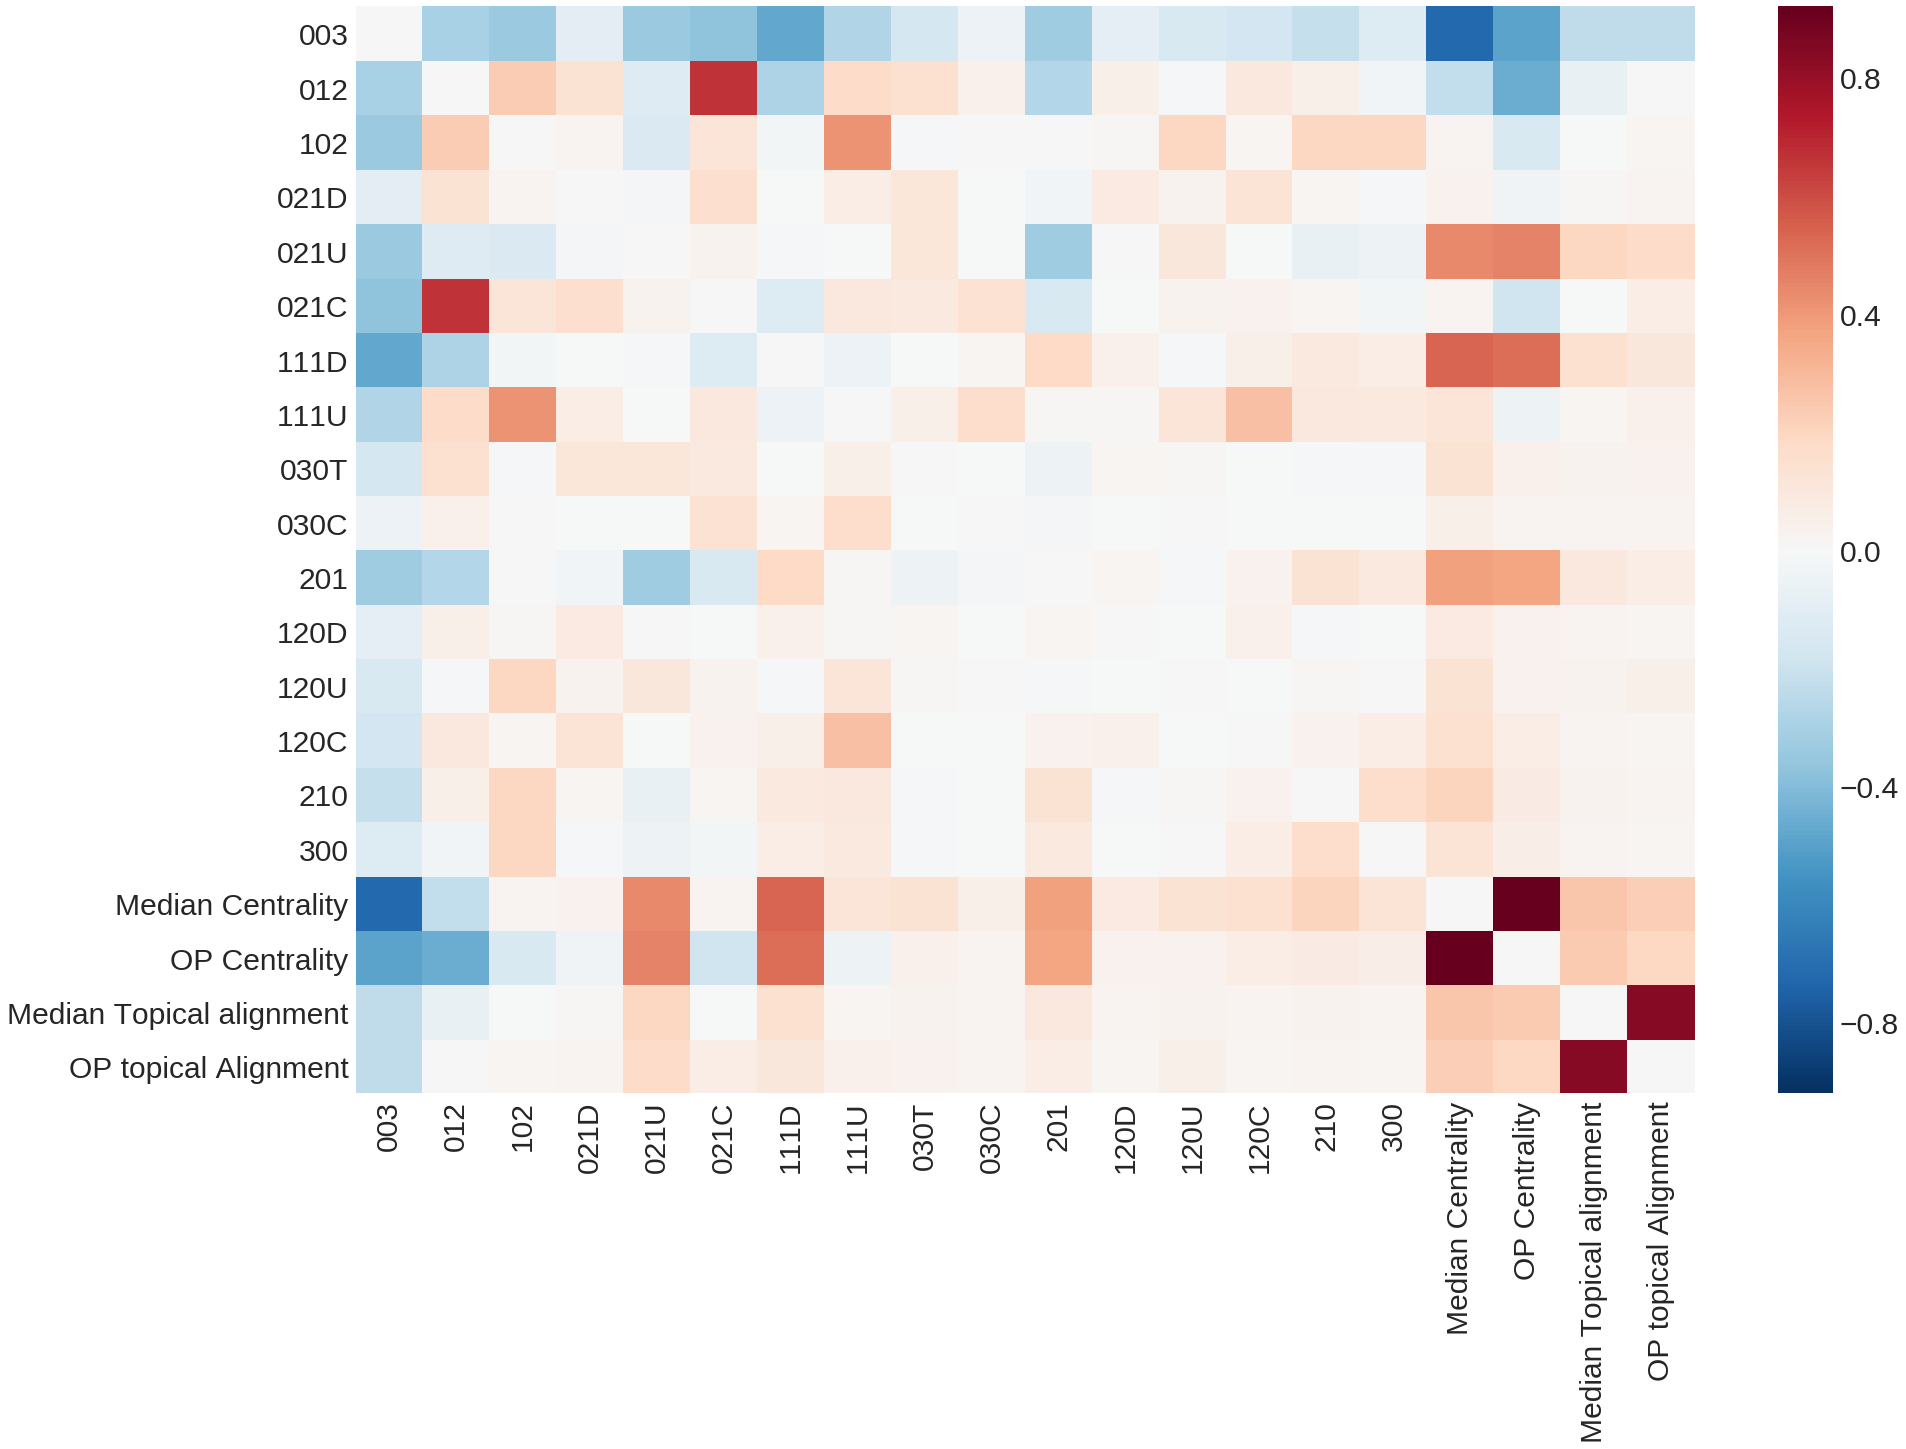
\includegraphics[width=0.5\linewidth, height = 6cm ]{Figures/normalized_corr.png}
% 		\label{fig:corrs}
% 	}
    
    \subfloat[]{
		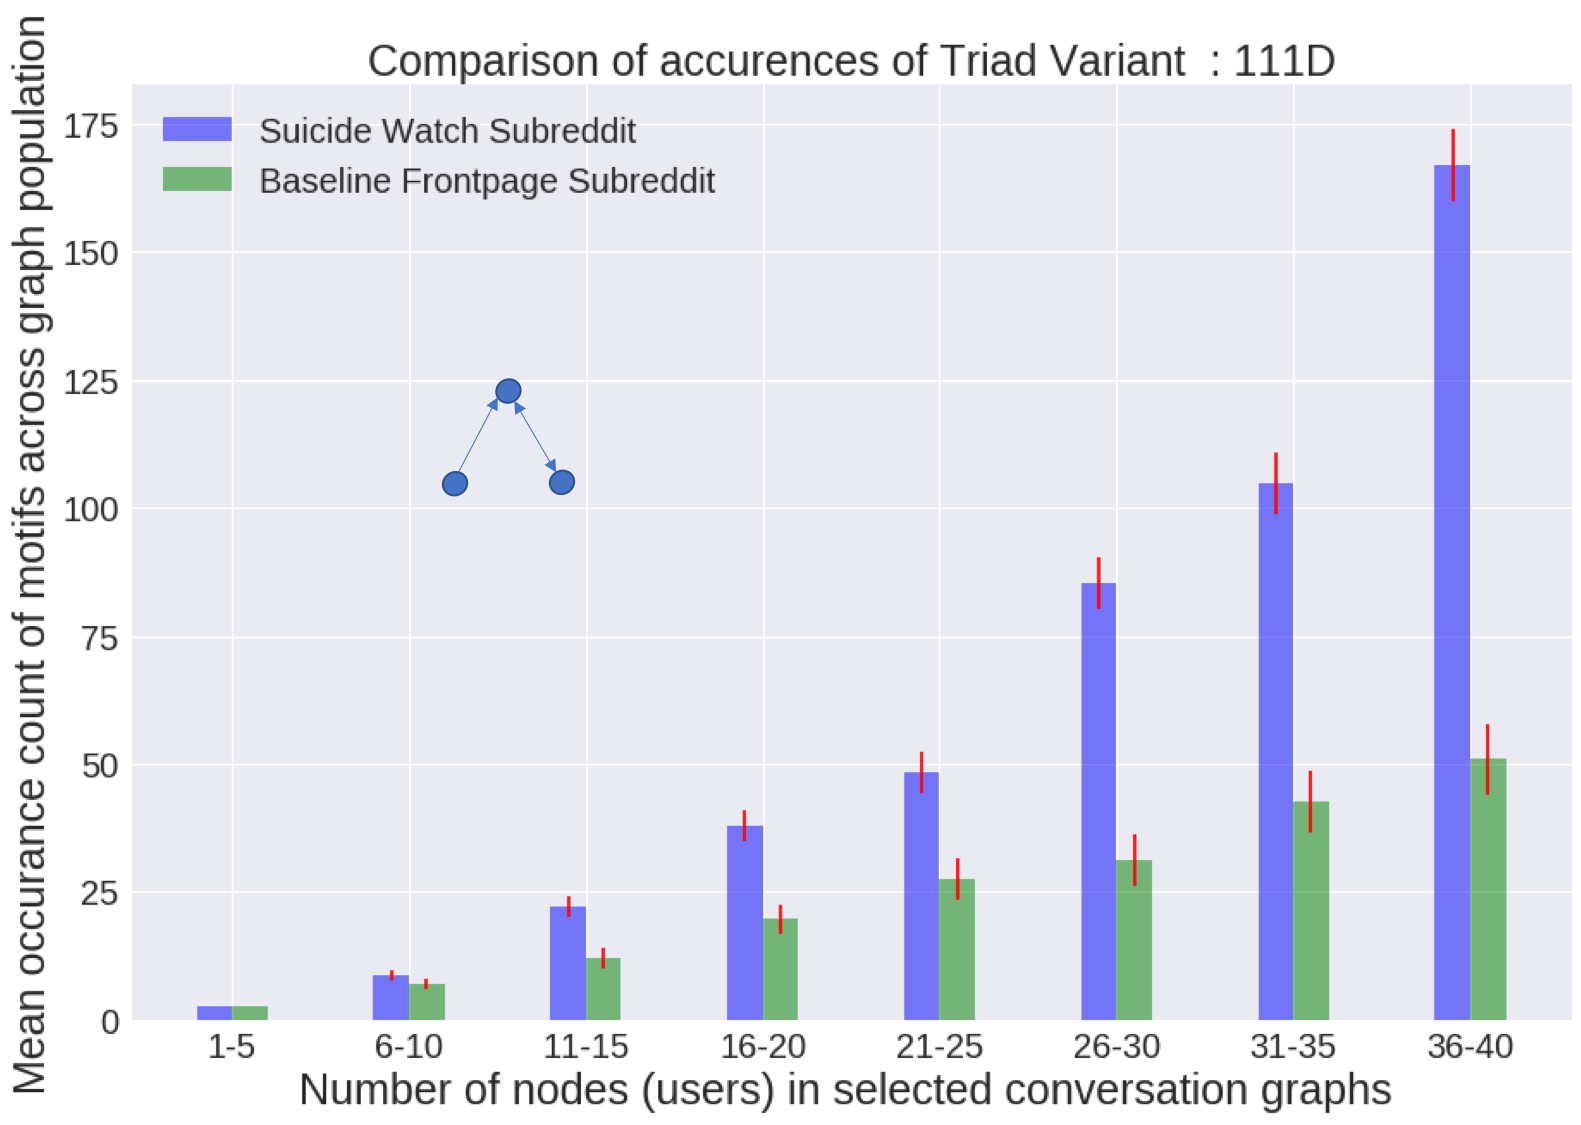
\includegraphics[width=0.5\linewidth ]{Figures/111D.png}
		\label{fig:111D_over}
	}
    \subfloat[]{
		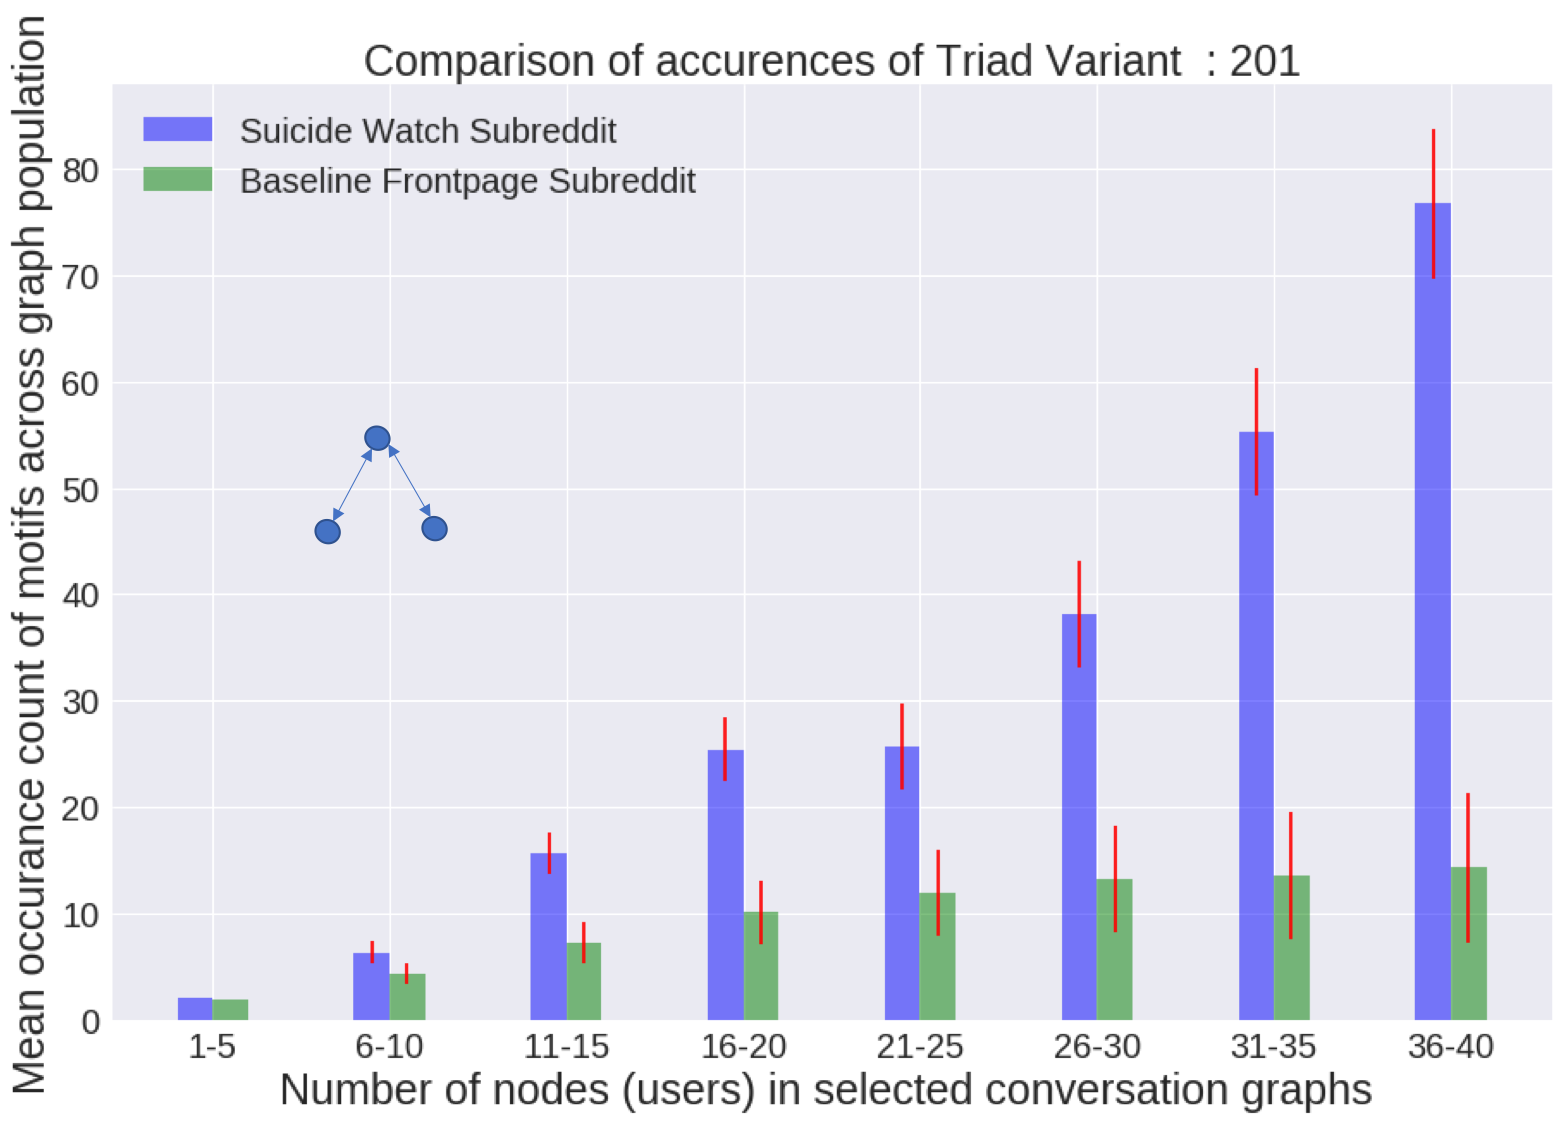
\includegraphics[width=0.5\linewidth ]{Figures/201.png}
		\label{fig:201_over}
	}
    
    \subfloat[]{
		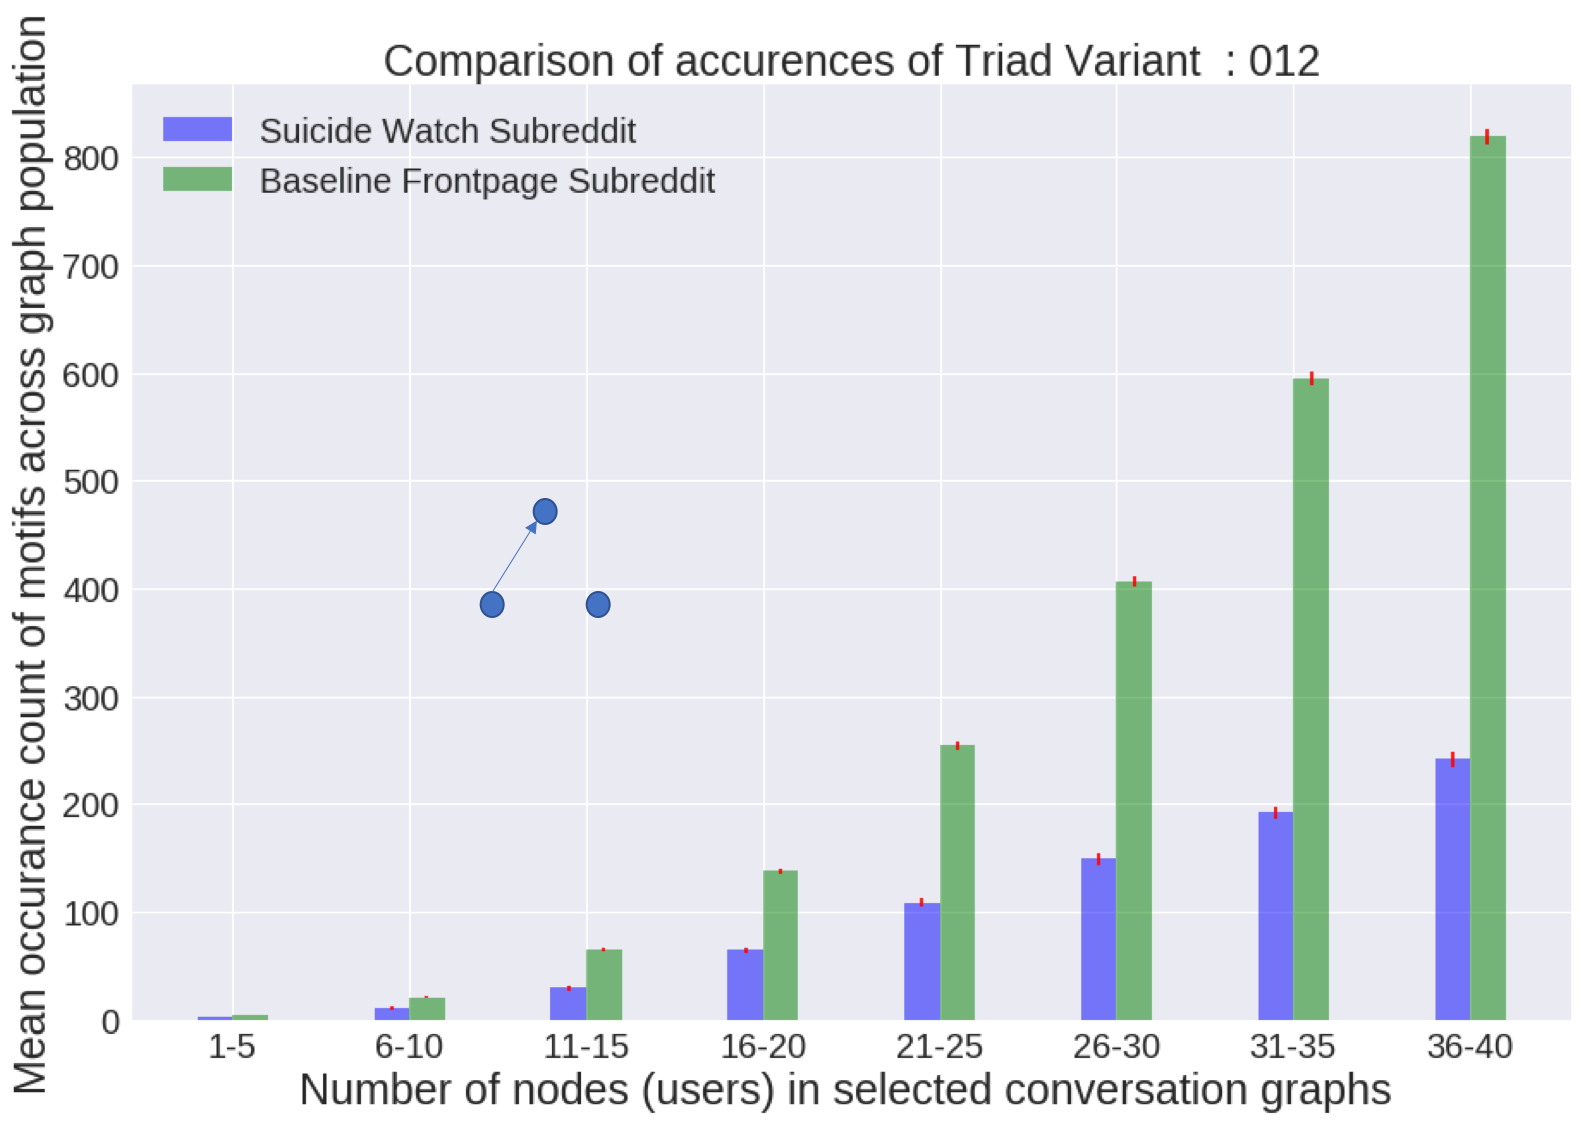
\includegraphics[width=0.5\linewidth ]{Figures/012.png}
		\label{fig:012_over}
	}
    \subfloat[]{
		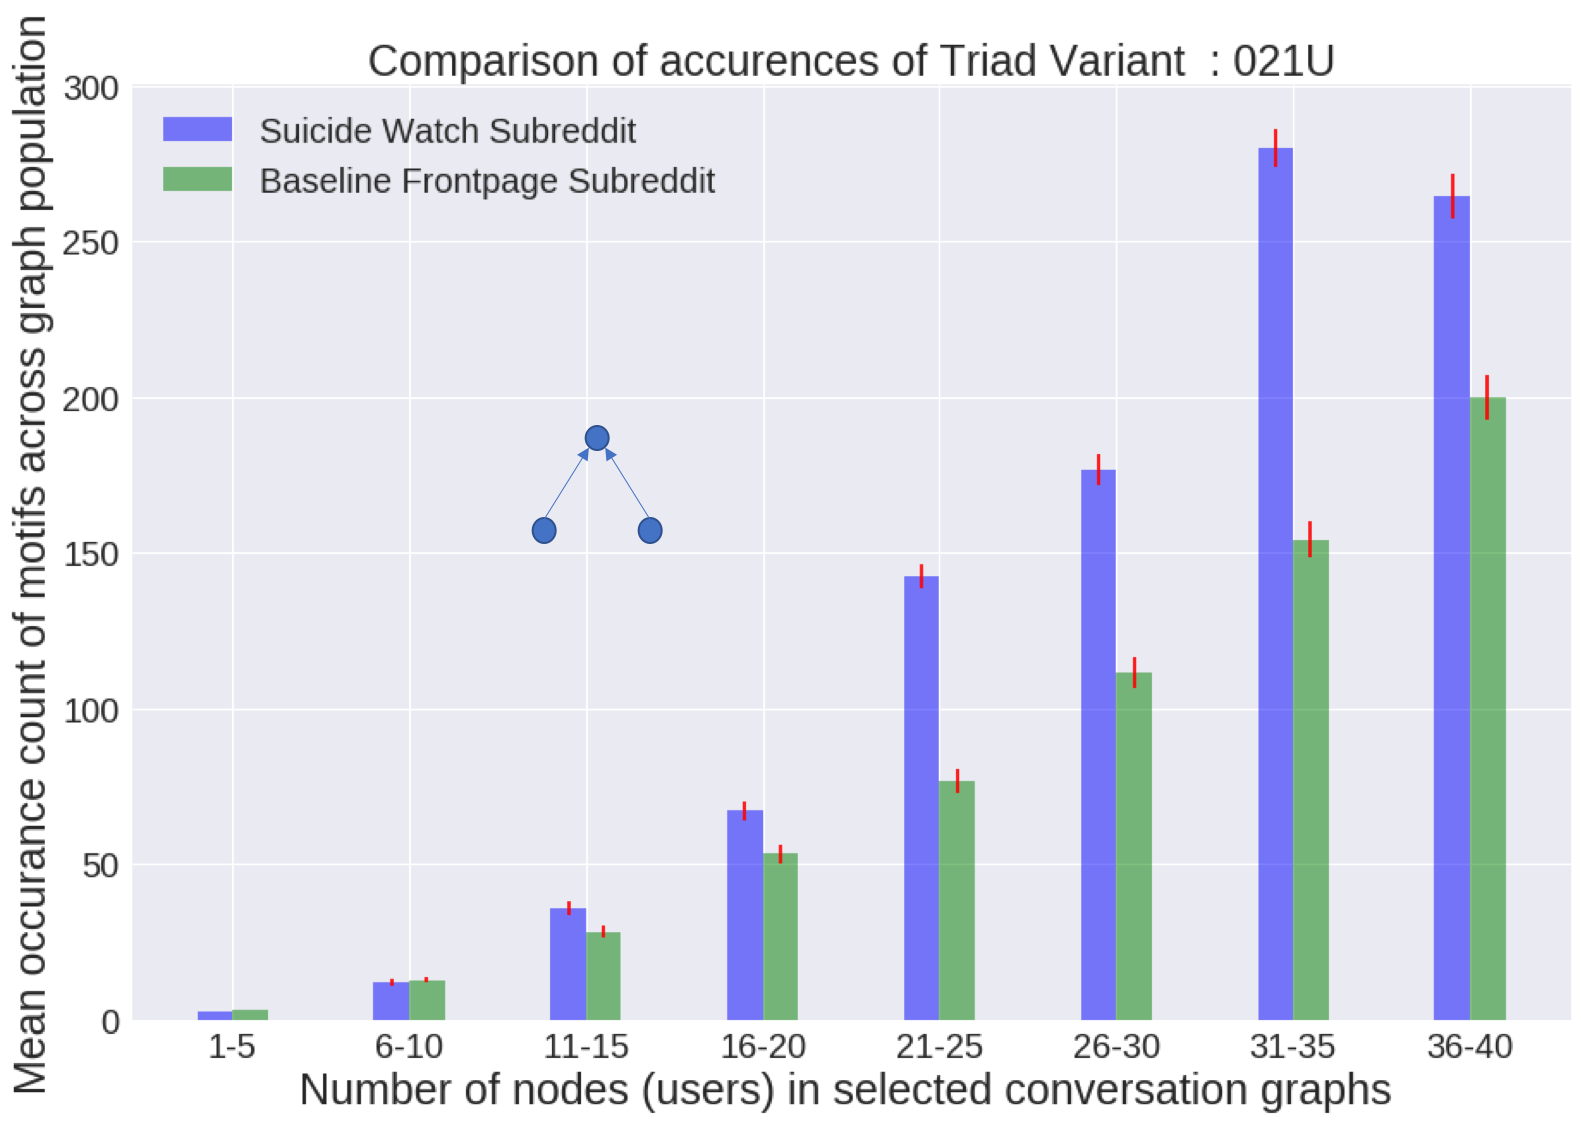
\includegraphics[width=0.5\linewidth ]{Figures/021U.png}
		\label{fig:021U_over}
	}
    
%    \subfloat[]{
%		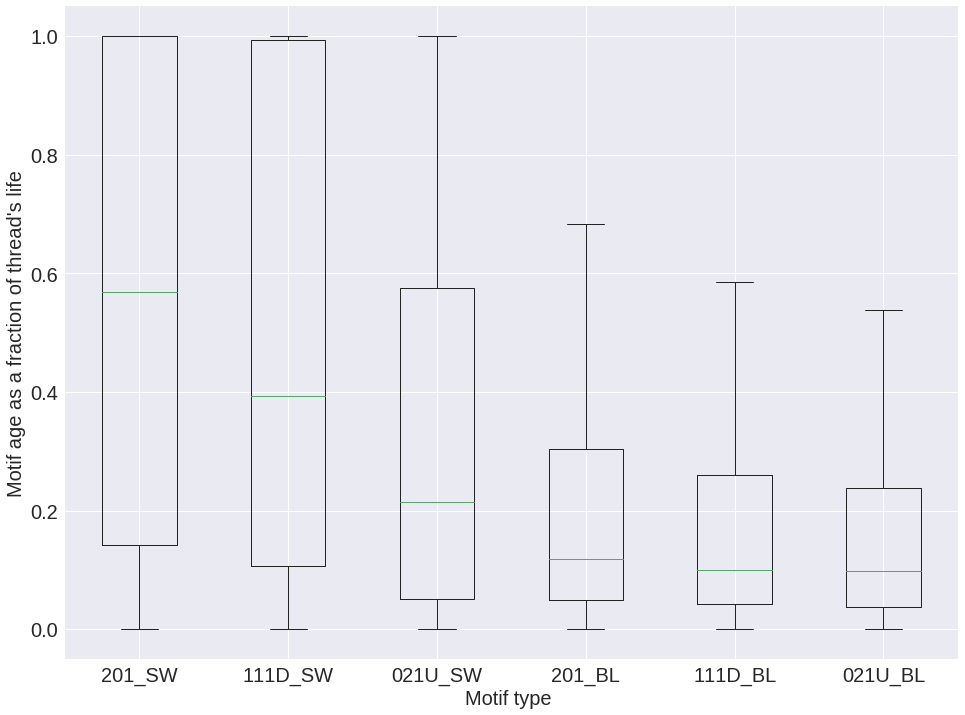
\includegraphics[width=0.5\textwidth, height = 6cm ]{Figures/BoxPlotMotifs_all.png}
%		\label{fig:motifOccurance}
%	}
%	\subfloat[]{
%		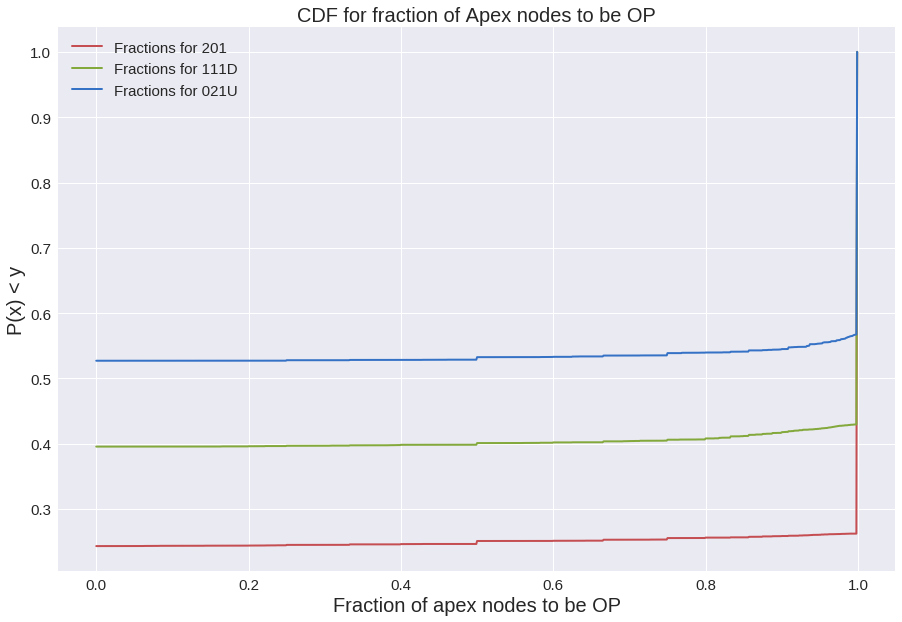
\includegraphics[width=0.5\linewidth, height = 6cm ]{Figures/CFD_ApexOP.png}
%		\label{fig:ApexOPProp}
%	}
    
    
\caption{This panel shows the statistical significance of the three over expressed and one under expressed triadic motif. 
%    Figure \ref{fig:motifOccurance} shows the distribution of each of the triadic motif's temporal point of occurrence according to the latest edge, as a proportion of the thread's lifetime. }
}
\end{figure}